
%(BEGIN_QUESTION)
% Copyright 2010, Tony R. Kuphaldt, released under the Creative Commons Attribution License (v 1.0)
% This means you may do almost anything with this work of mine, so long as you give me proper credit

En prosess patentert av Siemens for å danne staver av ultrarent silisium brukt som råstoff til solceller kalles ``TCS method.'' ``TCS'' står for tri-klor-silan, og er en gass med kjemisk formel HSiCl$_{3}$.

Prosessen bruker en silisiumtråd suspendert mellom to elektriske kontakter. Elektrisk strøm gjennom tråden varmer den opp til høy temperatur, og deretter slippes TCS-gass (pluss hydrogengass) inn i beholderen kalt ``CVD reactor'' (Chemical Vapor Deposition) ved et trykk på 6 bar (overtrykk). Der reagerer gassene på silisiumtråden og danner rent silisium (Si) og saltsyre (HCl), slik at silisium avsettes som nye lag på tråden. Etter hvert blir tråden tykkere til en massiv silisiumstav klar for videre prosessering. Syredamp forlater reaktoren sammen med ureaktert TCS og hydrogen:

$$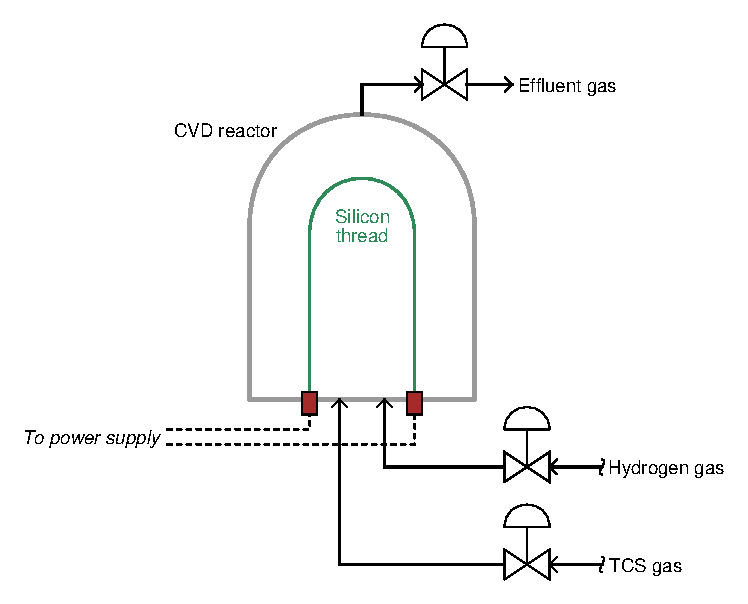
\includegraphics[width=15.5cm]{i00574x01.eps}$$

Balanser denne reaksjonsligningen for dannelse av nye silisiumlag inne i CVD-reaktoren:

$$\hbox{HSiCl}_3 + \hbox{H}_2 \rightarrow \hbox{Si} + \hbox{HCl}$$

Oppgi også gasstrykket i reaktoren i enheten PSIG.

\vskip 20pt \vbox{\hrule \hbox{\strut \vrule{} {\bf Forslag til sokratisk diskusjon} \vrule} \hrule}

\begin{itemize}
\item{} Ut fra prosessbeskrivelsen, tror du reaksjonen er eksoterm eller endoterm, eller er informasjonen for knapp til å si det?
\item{} Hvor sikkerhetsmessig risikable vil du vurdere noen av forbindelsene brukt i silisiumproduksjon, med tanke på menneskelig eksponering?
\end{itemize}

\underbar{file i00574}
%(END_QUESTION)





%(BEGIN_ANSWER)


%(END_ANSWER)





%(BEGIN_NOTES)

Denne reaksjonen er så enkel å balansere at algebra ikke er nødvendig. Det holder å ha {\it tre} syremolekyler på høyre side for å balansere tre hydrogenatomer og tre kloratomer på venstre side.

$$\hbox{HSiCl}_3 + \hbox{H}_2 \rightarrow \hbox{Si} + 3\hbox{HCl}$$

\vskip 10pt

6 bar (gauge) = 87 PSIG

\vskip 10pt

Informasjon til denne oppgaven er hentet fra Emersons ``Process Solutions Guide'' om Siemens TCS Method, dokumentnummer MC-001192.

%INDEX% Kjemi, støkiometri: reaksjonsmengder
%INDEX% Prosess: silanforbrenning

%(END_NOTES)

